\documentclass[a4paper,11pt]{article}
\usepackage[utf8]{inputenc}
\usepackage[spanish]{babel} %Idioma español
\usepackage[margin=30mm]{geometry} %Márgenes mas pequeños
\usepackage{hyperref} %Enlaces en la documentacion
\usepackage{graphicx} %Usar imagenes
\graphicspath{{./Resources/}}
\usepackage[numbib]{tocbibind} %Referencias aparecen en el indice
\usepackage{float} %Figuras[H]
%tabla
\usepackage{tabularx}
\usepackage{booktabs}

%opening
\title{
        \textbf{Cloud Foundry: PaaS}\large\\
        \textbf{Trabajo de curso}\\
        \medskip
        Universidad de Sevilla - Ingeniería Informática Tecnologías Informáticas\\
        Configuración, Implementación y Mantenimiento de Sistemas Informáticos\\
        Tercer curso}

\author{
Juan Arteaga Carmona\\ \href{mailto:JuanArteaga@andalu30.me}{JuanArteaga@andalu30.me}
\and
Rafael Dominguez Gonzalez\\ \href{mailto:rafadglez@hotmail.com}{rafadglez@hotmail.com}
\and
Aurora Gutierrez Martinez\\ \href{mailto:aurgutmar@alum.us.es}{aurgutmar@alum.us.es}
\and
Sergio Leon Riego\\ \href{mailto:serleorie@alum.us.es}{serleorie@alum.us.es}
\and
Francisco Pardillo Castillo\\ \href{mailto:blutonfenix@gmail.com}{blutonfenix@gmail.com}
}


\begin{document}

%Titulo
\maketitle

%Índices
\newpage
\tableofcontents
\listoffigures %Probablemente no lo vayamos a usar.

\renewcommand{\listtablename}{Índice de tablas} %Cambio de texto
\listoftables


\newpage



\section{Introducción}

\subsection{¿Qué es Cloud Foundry?}
Cloud Foundry es una plataforma que nos permite ejecutar aplicaciones, tareas y servicios. Al ser una plataforma cloud-native, utiliza infraestructura basada en la Nube de forma que las aplicaciones que son ejecutadas de la plataforma pueden estar aisladas de la configuración física, permitiendo así proveer de un servicio fiable de aplicaciones aún contando con una infraestructura no fiable.

\subsection{Plataformas en la nube}
Este tipo de plataformas nos permiten lanzar aplicaciones en red o servicios y hacerlos disponibles para todo el mundo en cuestión de minutos. Es un sistema flexible: cuando una apliación se vuelve popular, puede escalarse de forma sencilla para permitir más tráfico, simplificando un trabajo que antes podía requerir meses.
\begin{figure}[h]
    \centering
    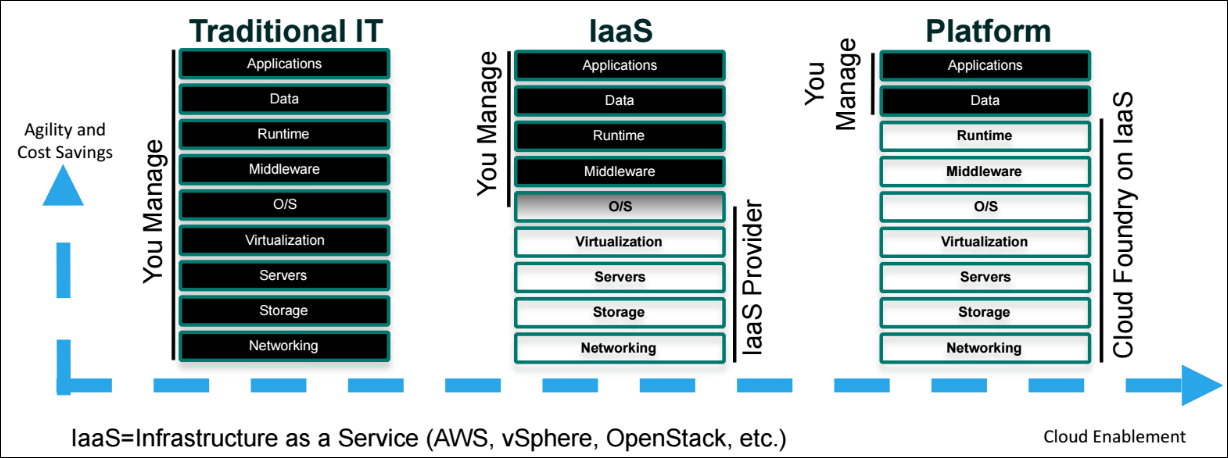
\includegraphics[width=0.85\textwidth]{power-of-platform.png}
    \caption{Evolución de las tecnologías de la información}
    \label{fig:powerplat}
\end{figure}


\subsection{¿Cómo funciona Cloud Foundry?}
Consta de subsistemas especializados en diferentes funciones:

\subsubsection{Balanceo de carga}
El sistema equilibra la carga de procesamiento en múltiples máquinas, optimizando eficiencia y fiabilidad. Se realiza a tres niveles:
\begin{enumerate}
  \item BOSH crea y lanza máquinas virtuales sobre una infraestructura física y, sobre ellas, ejecuta Cloud Foundry.
  \item  El Cloud Controller corre las aplicaciones y otros procesos en las máquinas virtuales, equilibrando la demanda y gestionando los ciclos de vida de las aplicaciones.
  \item El router enruta el tráfico entrante a las máquinas virtuales, generalmente funcionando con un balanceador de carga provisto por el cliente.
\end{enumerate}

\subsubsection{¿Cómo funcionan las aplicaciones?}
Cloud Foundry designa dos tipos de máquinas virtuales: las componentes, que constituyen la infraestructura de la plataforma, y las anfitrionas, que contienen las aplicaciones externas. El sistema Diego es el que regula la carga en estas últimas.

\subsubsection{¿Cómo organiza Cloud Foundry a los usuarios y entornos de trabajo?}
La gestión de los usuarios se realiza a través de dos servidores UAA (User Authentication and Authorization), que almacenan la información internamente o pueden conectarse a gestores externos de usuarios.

\subsubsection{¿Dónde almacena los recursos?}
Cloud Foundry utiliza el sistema git en GitHub para control de versiones de su código fuente, documentación y otros recursos. La plataforma utiliza bases de datos MySQL para el almacenamiento y compartición de archivos.

\subsubsection{Comunicación entre componentes}
La comunicación entre los diferentes elementos se realiza mediante mensajes internos utilizando protocolos http y https y mandando mensajes NATS entre ellos directamente.

\subsubsection{¿Cómo se monitoriza y analiza un sistema Cloud Foundry?}
La plataforma genera registros del sistema de cada uno de sus componentes y aplicaciones. El sistema Loggregator lo estructura y construye un sistema ordenado, llamado Firehose, a través del cual podemos monitorizar los servicios y generar alertas.


\section{Terminología básica}
 \begin{itemize}
 \item	AZ (Availability Zone): Un segmento de infraestructura de red funcionalmente independiente, a menudo correlacionado con la región geográfica, diseñado para aumentar la disponibilidad y la tolerancia a fallos.
 \item	Blob (Binary Large Objects, objetos binarios grandes): son elementos utilizados en las bases de datos para almacenar datos de gran tamaño que cambian de forma dinámica.
 \item	BOSH: es un proyecto de código abierto que ofrece herramientas para la implementación y la gestión del ciclo de vida de servicios distribuidos a gran escala.
 \item	CATs: CF Acceptance Tests (CATs). Está diseñado para probar características orientadas al usuario.
 \item	Cfdot (CF Diego Operator Toolkit): Herramienta diseñada para interactuar con los componentes de Diego.
 \item	Cloud controller: permite que los clientes accedan al sistema. Mantiene una base de datos con tablas para organizaciones, espacios, servicios, roles de usuario entre otros.
 \item	Cloud Foundry:  plataforma como servicio (PaaS) de código abierto originalmente desarrollado por VMware.
 \item	Diego: sistema de gestión de contenedores para Cloud Foundry.
 \item	Diego Brain: distribuye tareas y LRPs a Diego Cells y corrige las discrepancias entre los conteos reales y deseados para asegurar la tolerancia a fallos y la consistencia a largo plazo.
 \item	Docker: proyecto de código abierto que automatiza el despliegue de aplicaciones dentro de contenedores de software, proporcionando una capa adicional de abstracción y automatización virtualización de aplicaciones en múltiples sistemas operativos.
 \item	Dopplers: recopilan registros, los almacenan en buffers temporales y los envían a su destino.
 \item	Inigo: es una suite de prueba de integración que lanza los componentes de Diego a través de varios casos de prueba, incluyendo fallos de componentes y otros escenarios excepcionales.
 \item	Loggregator: recopila y transmite registros y métricas de aplicaciones de usuario en una implementación de Cloud Foundry, así como métricas de componentes de CF.
 \item	LRP (Long Running Process): procesos de larga duración.
 \end{itemize}



%Seccion Arquitectura - Juan Arteaga Carmona ---------------------
\section{Arquitectura}
\subsection{Introducción}
\label{sec:arquitectura}
La arquitectura de Cloud foundry se puede dividir en varias partes. A continuación se describirán los componentes mas importantes de cada una de estas partes.\\
En la figura \ref{fig:cuadroArquitectura}, ademas, se puede observar un esbozo simplificado de la arquitectura de CloudFoundry.

\begin{figure}[h]
    \centering
    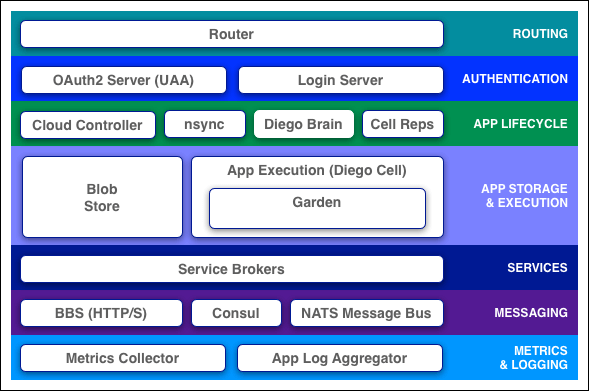
\includegraphics[width=0.75\textwidth]{cf_architecture_block}
    \caption{Estructura general de la arquitectura de Cloud Foundry}
    \label{fig:cuadroArquitectura}
\end{figure}

\subsection{Enrutamiento}
El router, también llamado Gorouter, es el encargado de enrutar el trafico entrante al componente adecuado, ya sea el CloudController o cualquier célula Diego, en la que como veremos más adelante se ejecutan las aplicaciones. Este router esta implementado en Go, lo que hace que tenga control total sobre cada conexión, lo que simplifica el soporte para otros tipos de tráfico no clásico como WebSockets y HTTP CONNECT.
Toda la lógica de enrutamiento se lleva a cabo en un proceso independiente, lo que hace que se reduzca la latencia.\\
El router recibe la información de las actualizaciones a traves del sistema de mensajería NATS de CloudFoundry, en concreto mediante queries al Diego Bulletin Board System (BSS), que le indica en que células y contenedores se encuentran que aplicaciones. Si estos enrutamientos no se ven actualizados en dos minutos se ven eliminados, por lo tanto el proceso de queries al BBS se realiza al menos una vez cada dos minutos.


\subsection{Autentificación}
El servidor de OAuth, comúnmente llamado el UAA, y el servidor de inicio de sesión trabajan para asegurar la autentificación.\\
El papel principal del UAA es el de proveedor de OAuth2, dar tokens a aplicaciones. Junto con el servidor de inicio de sesión, el UAA autorizará a los usuarios con las credenciales de CF o con cualesquiera que hayan sido configuradas.

\subsection{Ciclo de vida de la aplicación}
\subsubsection{Cloud Controller y Diego Brain}
El Cloud Controller es el encargado de dirigir el despliegue de las aplicaciones. Es el endpoint al que se conectan los desarrolladores que quieren desplegar una aplicación en CF. El CC necesita de una base de datos Postgres o MySQL.\\
El CC conectará con el DiegoBrain, que como su nombre indica, es el cerebro principal del sistema Diego, que como veremos en la sección \ref{sec:DiegoCell}, es el encargado de poner en funcionamiento las VMs necesarias para que la aplicación funcione tal y como la quiere el usuario.

\subsubsection{nsync, BSS, Cell Reps}
Estos componentes son los que hacen que las aplicaciones se mantengan funcionando. Son los responsables de monitorizar y analizar los estados de los contenedores así como iniciarlos y pararlos para cumplir con las especificaciones del usuario.

\begin{itemize}
  \item \textbf{nsync} es el encargado modificar el parámetro `DesiredLRP' en la BSS de Diego.
  \item \textbf{Cell Rep} es el encargado de actualizar el parámetro `ActualLRP' en la BSS con el valor correcto.
  \item \textbf{BSS} es la base de datos de Diego, la cual se encarga de que los dos parámetros anteriores sean iguales. Puede modificar el numero de contenedores para que esta igualdad se mantenga siempre.
\end{itemize}


\subsection{Almacenamiento y ejecución de la aplicación}
\subsubsection{Blobstore}
El blobstore es un repositorio para archivos binarios grandes los cuales Github no sería capaz de almacenar eficientemente.

\subsubsection{Diego Cell}\label{sec:DiegoCell}
Todas las aplicaciones que se ejecutan en CF se ejecutan dentro de unos contenedores llamados Garden, dentro de las maquinas virtuales conocidas como Diego Cells. Las Diego Cells son las que se encargan de mantener los contenedores funcionando así como de reportar su estado al Diego BSS y de enviar los logs a Loggregator, que como veremos a continuación es el encargado de hacer llegar los logs de los contenedores a los usuarios.

\subsection{Métricas y Logs}
\subsubsection{Loggregator}
El Loggregator, de la unión de las palabras inglesas `log' y `aggregator' es el encargado de hacer llegar los logs de las aplicaciones a los usuarios.
\subsubsection{Recolector de métricas}
El recolector de métricas se encarga de recoger las métricas de los distintos componentes de CF, lo que permite monitorizar el despliegue de CF así como aplicar una mejora continua a la infraestructura.

%-----------------------------------------------------------------



\section{Distribución}%Aurora
Podemos distinguir entre dos sistemas: distribuidos y en red.

\subsection{Sistemas distribuidos vs Sistemas en red}
\begin{itemize}
  \item  Sistemas distribuidos: es un conjunto de computadores separados físicamente y conectados entre sí por una red de comunicaciones distribuida; cada máquina posee sus componentes de hardware y software que el usuario percibe como un solo sistema.
  \item Sistemas en red: Es aquel que utiliza los recursos de una sola computadora central, es decir, su memoria, CPU, disco y periféricos. La computadora en sí misma puede controlar todos los periféricos directamente (si están físicamente conectados con la
computadora central), o conectados a través de un servidor de terminal.
\end{itemize}

Ventajas de los sistemas distribuidos:
\begin{itemize}
  \item Económicos
  \item Trabajo en conjunto
  \item Mayor confiabilidad
\end{itemize}

Ventajas de los sistemas en red:
\begin{itemize}
  \item Mejor aprovechamiento de los recursos individuales.
  \item Mayor poder de cómputo a menor precio.
  \item Menor redundancia.

\end{itemize}

\subsection{Cloud Foundry como sistema distribuido}
Diego es un sistema distribuido que le permite ejecutar y escalar N cantidad de aplicaciones y tareas en contenedores a través de una cantidad de celdas. Aquí están las principales características y atributos de Diego:
\begin{itemize}
  \item Es responsable de ejecutar y monitorear las imágenes compatibles con OCI, las aplicaciones independientes y las tareas implementadas en Cloud Foundry.
\item Al residir en el núcleo de Cloud Foundry, Diego se encarga de la programación, ejecución y supervisión de tareas y procesos de larga ejecución (aplicaciones) que residen dentro de contenedores administrados.
\item Es agnóstico tanto para la interacción del cliente como para la implementación en tiempo de ejecución.
\item Asegura que las aplicaciones sigan ejecutándose al conciliar el estado deseado con el estado real mediante el establecimiento de una consistencia eventual, la recuperación automática y los ciclos de retroalimentación cerrados.
\item Cuenta con un entorno de ejecución genérico compuesto de acciones y backends para permitir el soporte de múltiples cargas de trabajo diferentes basadas en Windows y Linux.
\end{itemize}

Cuando da un paso atrás y considera los desafíos inherentes con cualquier sistema distribuido, las soluciones a los desafíos de coherencia y orquestación proporcionados por Diego son extremadamente elegantes. Diego ha sido diseñado para hacer que el subsistema de tiempo de ejecución de contenedores de Cloud Foundry sea modular y
genérico.\\
La mayoría de los usuarios de Cloud Foundry (por ejemplo, desarrolladores) no interactúan con Diego directamente. Los desarrolladores interactúan solo con la API de Cloud Foundry,
conocida como CAPI. Sin embargo, comprender el tiempo de ejecución del contenedor de Diego es esencial para los Operadores de Plataforma porque, como operador, debe interactuar con Diego por consideraciones clave, como los requisitos de resistencia y la resolución de problemas de las aplicaciones.

\subsection{La importancia de la gestión de contenedores}
Para que una imagen de contenedor (como una imagen compatible con OCI) se ejecute como un proceso aislado, se requiere una capa de administración de contenedor que pueda crear, ejecutar y administrar el proceso de contenedor. Como una API de administración de
contenedores más generalizada, Cloud Foundry usa Garden para admitir una variedad de tecnologías de contenedores.\\

A través de Garden, Diego ahora puede admitir cualquier formato de imagen de contenedor que admita la API de Garden. Además, también ha agregado soporte para ejecutar contenedores en cualquier tecnología de contenedor basada en Garden, incluidos los backends de contenedor basados en Linux y Windows que implementan la API de Garden. La figura \ref{fig:capacidadDiego} ilustra la capacidad de Diego para admitir múltiples artefactos de aplicación y formatos de imagen de contenedor.

\begin{figure}[H]
    \centering
    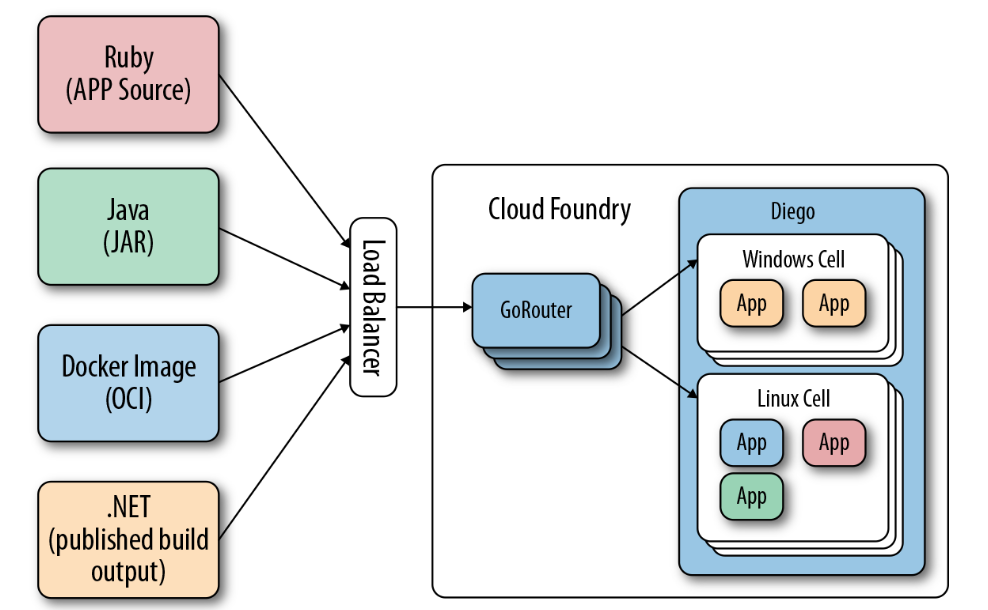
\includegraphics[width=0.75\textwidth]{aurora1.png}
    \caption{Capacidad de Diego para admitir múltiples artefactos de aplicación y formatos de imagen de contenedor}
    \label{fig:capacidadDiego}
\end{figure}


\subsection{Arquitectura de Diego}
Diego está compuesto por varios microservicios que residen en varios componentes, como puede verse en la figura \ref{fig:arqDiego}.
\begin{figure}[h]
    \centering
    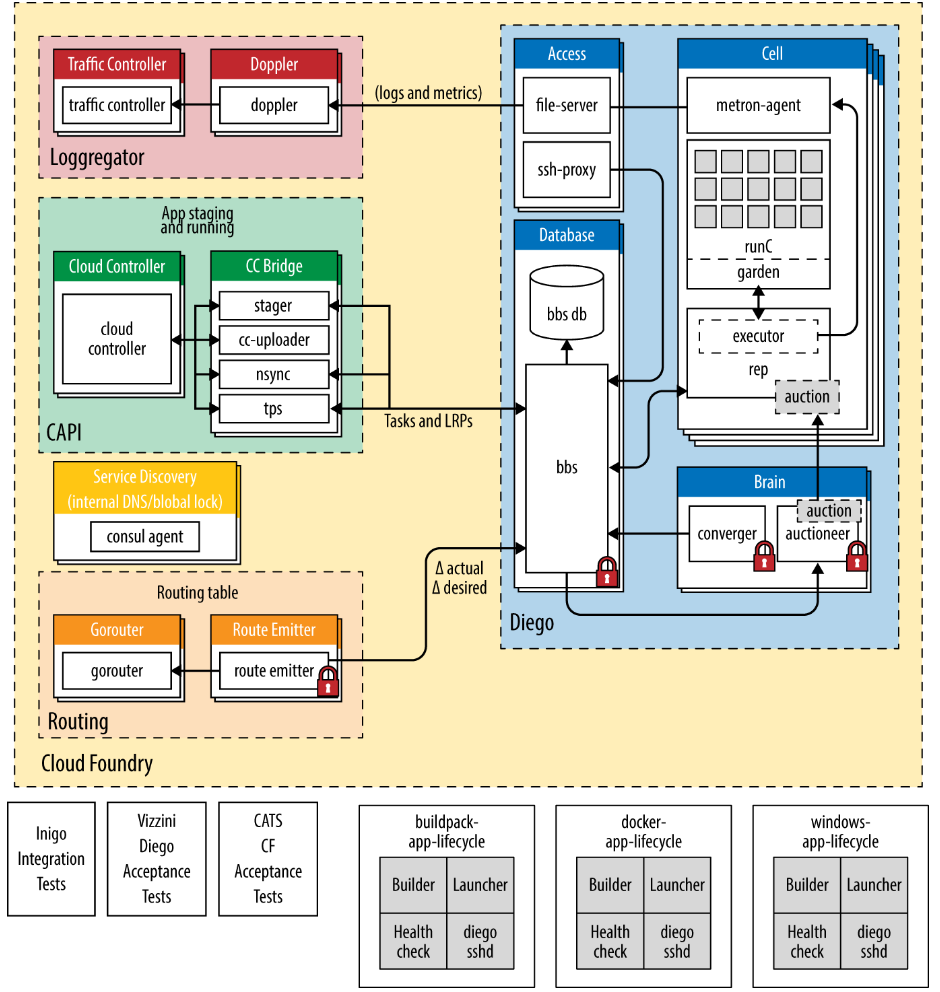
\includegraphics[width=0.75\textwidth]{aurora2.png}
    \caption{Microservicios que componen Diego}
    \label{fig:arqDiego}
\end{figure}
Podemos agrupar los componentes, ampliamente, de la siguiente manera:
\begin{itemize}
  \item  Una capa de Cloud Foundry de componentes orientados al usuario (componentes con los que el usuario de la plataforma, interactuará directamente).
\item  La capa de Diego Container Runtime (componentes con los que interactúan los componentes centrales de Cloud Foundry).
\end{itemize}

\subsection{Interactuando con Diego}
Los usuarios de Cloud Foundry no interactúan con Diego directamente; interactúan con los componentes orientados al usuario de Cloud Foundry, que luego interactúan con Diego en nombre del usuario. Aquí están los componentes orientados al usuario de Cloud Foundry que funcionan en conjunto con Diego:
\begin{itemize}
  \item  Componentes CAPI: la API de Cloud Foundry (Cloud Controller y el CC-Bridge).
\item  El sistema de registro definido por los agentes Loggregator y Metron.
\item  Enrutamiento (GoRouter, TCPRouter y el Emisor de ruta).
\end{itemize}
En conjunto, estos componentes de Cloud Foundry son responsables de lo siguiente:
\begin{itemize}
  \item Política de aplicación.
\item  Cargar artefactos, droplets y metadatos de la aplicación en un blobstore.
\item  Tráfico de enrutamiento y manejo de tráfico de aplicaciones.
\item  Gestión de usuarios, incluida la interacción del usuario final a través de los comandos
de API de Cloud Foundry.
\end{itemize}
Diego se conecta sin problemas a estos diferentes componentes de Cloud Foundry para ejecutar aplicaciones y tareas, enrutar el tráfico a sus aplicaciones y permitir la recuperación de los registros necesarios.






%------------------------------------------------------------------
\section{Escalado}
El escalado es necesario siempre que queramos que nuestras aplicaciones sean capaces de manejar un mayor número de usuarios al mismo tiempo, despachar un mayor número de solicitudes en paralelo, etc.\\
En definitiva, con el escalado lo que se busca es aumentar la capacidad y la disponibilidad de nuestra plataforma, así como reducir las posibilidades de tiempo de inactividad.\\
En Cloud Foundry PaaS disponemos de 2 tipos de escalado:

\subsection{Escalado horizontal}
El escalado horizontal de una aplicación consiste en aumentar el número de instancias en ejecución para una determinada aplicación desplegada en la nube Cloud Foundry.\\
El escalado horizontal puede ser positivo o negativo, esto es crear nuevas instancias de la aplicación o destruir instancias existentes de la misma.\\
Para escalar horizontalmente, se utiliza el siguiente comando:\\
\begin{itemize}
  \item cf scale APP -i INSTANCES
  \item cf scale myApp -i 5
\end{itemize}
Donde “INSTANCES” es el número de instancias y “APP” es el nombre de la aplicación la cual queremos escalar.\\
En el ejemplo podemos apreciar cómo se le asignan 5 instancias a la aplicación “myApp”.\\

\subsection{Escalado vertical}
El escalado vertical de una aplicación en Cloud Foundry consiste en variar/modificar las prestaciones que las instancias de la aplicación tiene atribuidas.\\
Esto nos permitirá limitar el espacio en disco que Cloud Foundry atribuye a las instancias de una determinada aplicación, el límite de memoria que se le aplica a las instancias, etc.\\
Para escalar verticalmente se utiliza una variación del comando de escalado horizontal. Veámoslo con unos ejemplos:\\
\begin{itemize}
\item cf scale APP -k DISK
\item cf scale myApp -k 512M
\end{itemize}
Aquí podemos ver como limitamos la cantidad de disco que Cloud Foundry le asigna a las instancias de la aplicación “myApp”, limitándola a una cantidad igual a 512 Megabytes de disco usado para cada instancia de dicha aplicación
\begin{itemize}
\item cf scale myApp -k 512M
\item cf scale myApp -m 1G
\end{itemize}
Aquí podemos ver como limitamos la cantidad de memoria que Cloud Foundry le asigna a las instancias de la aplicación “myApp”, limitándola a una cantidad igual a 1 Gigabyte de memoria usado para cada instancia de dicha aplicación.

\subsection{Acerca del comando ``SCALE''}
Nos permite ver o cambiar el recuento de instancias, el límite de espacio en disco y el límite de memoria para una aplicación.
\begin{verbatim}
cf scale APP_NAME [-i INSTANCES] [-k DISK] [-m MEMORY] [-f]
\end{verbatim}
\begin{itemize}
  \item f: Nos permite forzar el reinicio de la aplicación sin aviso.
    \item i: Número de instancias
    \item k: límite de disco que se usa para cada instancia de la aplicación (por ejemplo, 256M, 1024M, 1G).
    \item m: límite de memoria que se usa para cada instancia de la aplicación (por ejemplo, 256M, 1024M, 1G).
\end{itemize}
Hay que tener en cuenta que el hecho de escalar una aplicación a 5 instancias y 32GB de memoria, implica que cada una de las 5 instancias tendrá como límite 32GB de memoria, y no que cada una de las 5 instancias tenga 32/5(GB) como límite de memoria.

\subsection{Escalado de los componentes de una implementación ded Cloud Foundry y concepto e ``AZ'' (Zonas de disponibilidad)}
Lo cierto es que las aplicaciones que desplegamos en nuestra nube Cloud Foundry no es lo único que puede ser escalable.
Otro aspecto que puede escalarse son los propios componentes de la implementación de una nube Cloud Foundry.

\begin{figure}[h]
    \centering
    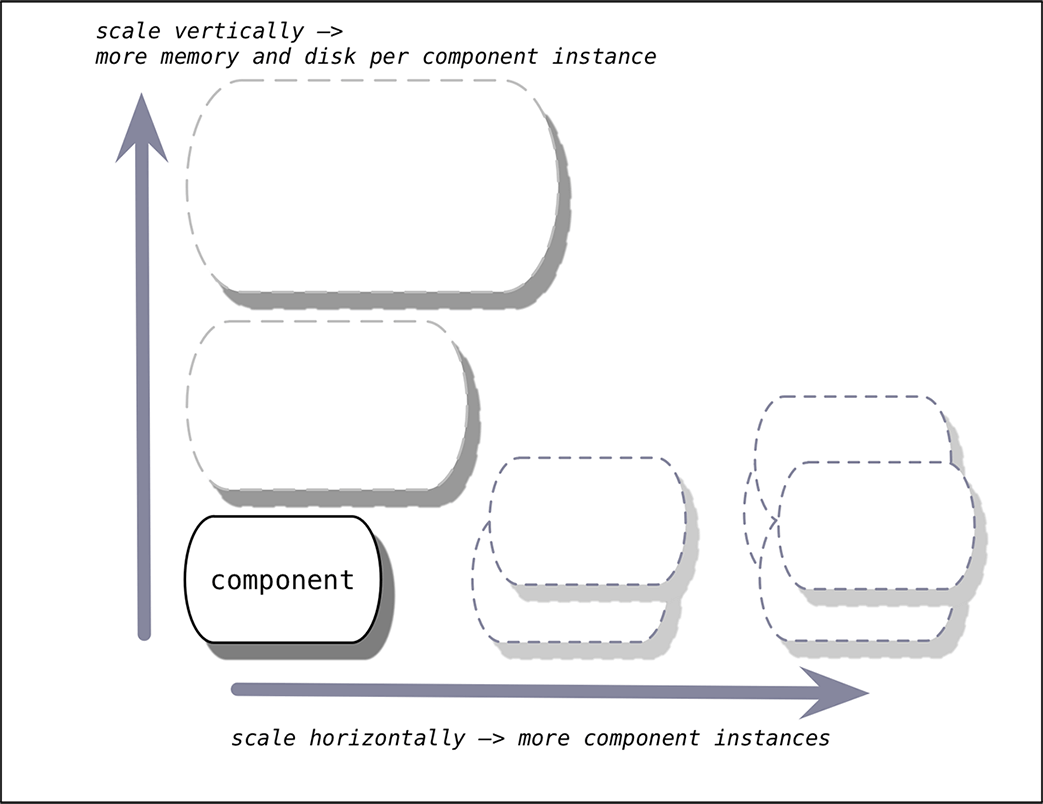
\includegraphics[width=0.75\textwidth]{fran1.png}
    \caption{Tipos de escalado}
    \label{fig:fran1}
\end{figure}

Es decir, hablamos de escalar la plataforma en sí misma, escalar la implementación de Cloud Foundry a través del escalado de sus componentes, donde el escalado horizontal implicará la creación de un mayor número de máquinas virtuales (VM’s) que ejecuten nuevas instancias de los componentes de la plataforma.
Es por ello que una ampliación horizontal para ciertos componentes tiene como implicación el aumentar la capacidad de alojar aplicaciones.\\
El vertical agregará memoria y disco a cada instancia del componente, tal y como lo hace el vertical sobre las aplicaciones.
A la hora de hacer un escalado vertical, se ha de considerar:
\begin{itemize}
  \item Tener suficiente espacio libre existente en las celdas del subsistema Diego de las máquinas virtuales anfitrionas para que las aplicaciones que se espera que se desplieguen se puedan organizar y ejecutar con éxito (Son en las celdas de Diego donde se aceptan y ejecutan las tareas e instancias de “Long Running Process” [LRP] de las diferentes aplicaciones que se ejecutan en la nube).
\item Una asignación suficiente de espacio en disco y memoria en su implementación de tal manera que, si una máquina virtual anfitriona está inactiva, todas las instancias de aplicaciones se pueden colocar en las máquinas virtuales host restantes.
\item El espacio libre para manejar una AZ (zona de disponibilidad) cae/baja si se hace un despliegue/implementación en múltiples AZ.
\end{itemize}
El escalado de componentes de una implementación de Cloud Foundry surge a partir de los riesgos que tiene la venida abajo de una de las AZ (zonas de disponibilidad) que componen la implementación de la nube de Cloud Foundry.

Lo cierto es que cuando se producen updates de productos o upgrades en la plataforma, es frecuente que alguna de las máquinas virtuales VM’s que ejecutan instancias, se venga abajo haciéndola temporalmente inasequible.

Es por ello que una correcta distribución de los componentes de la implementación de la nube Cloud Foundry a través de las distintas Zonas de Disponibilidad que la compongan y su correspondiente escalado a un nivel suficiente de redundancia garantizará una alta disponibilidad tanto durante las actualizaciones como durante las interrupciones y con ello se puede garantizar un tiempo de inactividad con tendencia al 0.

La implementación de Cloud Foundry en tres o más AZ y la asignación de múltiples instancias de componentes a diferentes ubicaciones de AZ permiten que una implementación funcione sin interrupciones cuando alguna de las AZ queda inoperable.
Cloud Foundry mantendrá su disponibilidad mientras la mayoría de las AZ sigan siendo accesibles. Por ejemplo, una implementación de tres AZ se mantiene en alto cuando una AZ completa se cae, y una implementación de cinco AZ puede soportar una interrupción de hasta dos AZ sin afectar en el tiempo de actividad.

\subsection{Autoescalador}
En caso de que usemos el proveedor Pivotal Software para Cloud Foundry, dispondremos de una aplicación para auto escalar aplicaciones integrada en la interfaz de usuario Apps Manager.\\
Esto ayudará a controlar el coste de ejecutar aplicaciones mientras se mantiene el rendimiento de la aplicación. Para equilibrar el rendimiento y el coste de la aplicación, se puede utilizar esta aplicación para lo hacer lo siguiente:
\begin{itemize}
  \item Configurar reglas que ajusten los recuentos de instancias según los umbrales de las métricas, como el uso de la CPU.
  \item Modificar el número máximo y mínimo de instancias para una aplicación, ya sea manualmente o siguiendo un programa.
\end{itemize}
Para usar la aplicación de auto escalar, se debe crear una instancia del servicio “App Autoscaler” y vincularla a cualquier aplicación que queramos escalar automáticamente.\\
Una vez hecho esto, nos vamos al administrador de aplicaciones (App Manager) y desde ahí seleccionamos una de las aplicaciones del espacio en el que se creó el servicio autoscaler de la aplicación (la instancia anteriormente mencionada)\\
Como paso siguiente, nos vamos a la pestaña “Procesos e instancias” y activamos el botón “Autoscaling”.
\begin{figure}[H]
    \centering
    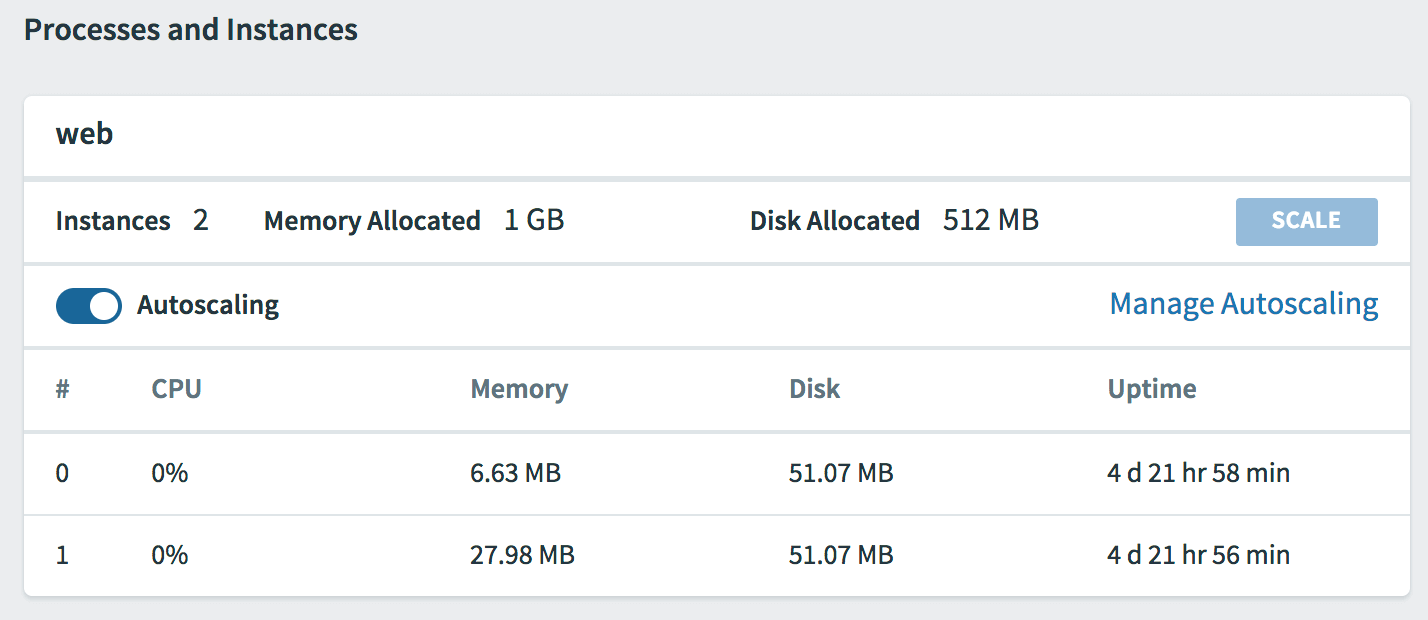
\includegraphics[width=0.75\textwidth]{fran2.png}
    \caption{Administrador de autoescalado}
    \label{fig:fran2}
\end{figure}
Desde la pestaña de administración de auto escalado, “Manage Autoscaling”, podemos limitar el número mínimo y máximo de instancias de la aplicación.\\
Si en algún momento decidimos apostar otra vez por escalar manualmente una aplicación la cual anteriormente hayamos vinculado a una instancia del servicio de auto escalado, se desactivará el auto escalado que hayamos configurado. Cuidado con esto.
Para mantener las aplicaciones disponibles sin desperdiciar recursos, la aplicación Autoscaler incrementa o disminuye el número de instancias en base a una comparación que lleva a cabo entre la métrica (CPU, RAM, disco, etc.) y el umbral mínimo/máximo establecido para dicha métrica.\\
La aplicación Autoscaler escala las aplicaciones de la siguiente manera:
\begin{itemize}
  \item Incremento en una instancia cuando cualquier métrica excede el umbral máximo especificado.
  \item Disminuye en una instancia solo cuando todas las métricas caen por debajo del umbral mínimo especificado.
\end{itemize}
Algunas métricas en las que podemos basarnos para crear las reglas del auto escalador de aplicaciones:
\begin{itemize}
  \item Uso de la CPU: Porcentaje de CPU promedio para todas las instancias de la aplicación.
  \item Utilización de memoria de un contenedor: Porcentaje de memoria promedio para todas las instancias de la aplicación.
  \item Utilización de memoria de un contenedor: Porcentaje de memoria promedio para todas las instancias de la aplicación.
\end{itemize}
\begin{figure}[H]
    \centering
    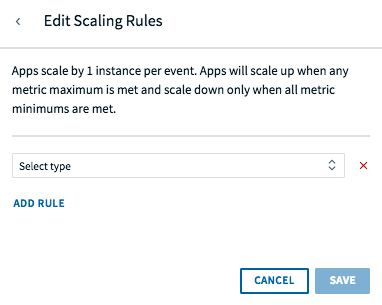
\includegraphics[width=0.75\textwidth]{fran3.png}
    \caption{Añadir reglas basadas en métricas}
    \label{fig:fran3}
\end{figure}
Debido a que la demanda de aplicaciones a menudo sigue un programa semanal, diario o por horas, se puede programar la aplicación Autoscaler para que cambie el rango de instancias permitido para seguir los aumentos esperados o los períodos de inactividad que se presuponen, ya que sabemos que la demanda de la aplicación difiere según el momento.
\begin{itemize}
  \item Fecha y hora: establezca la fecha y la hora del cambio de número de instancias.
  \item Repetir: establezca el día de la semana en el que desea repetir el cambio.
  \item Mínimo y máximo: Establezca el rango permitido dentro del cual App Autoscaler puede cambiar el número de instancias para una aplicación.
\end{itemize}
\begin{figure}[H]
    \centering
    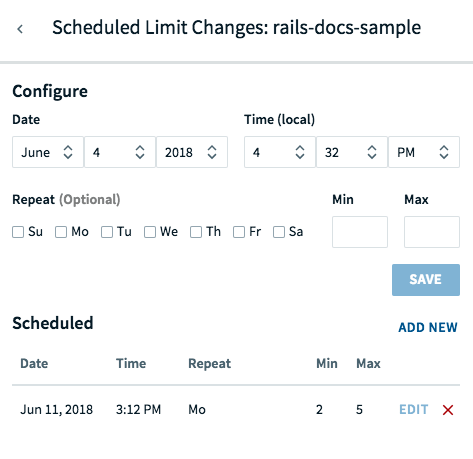
\includegraphics[width=0.75\textwidth]{fran4.png}
    \caption{Configurando horarios para el escalado}
    \label{fig:fran4}
\end{figure}
También existen otras opciones de código abierto como app-autoscaler y cf-autoscaler.


%------------------------------------------------------------------
\section{Replicación}

\subsection{Introducción a la replicación}
La replicación es totalmente necesaria en sistemas de la información, ya que nos garantiza mayor fiabilidad y protección ante fallos, ataques o desastres, al clonarse las instancias desplegadas. En caso de bases de datos, ademós, nos permite mayor acceso en paralelo, pues es más habitual la lectura de información que la escritura.

\subsection{Replicaciónn en Cloud Foundry}
Cloud Foundry permite la creación de múltiples instancias redundantes que garanticen la resiliencia y demandas de disponibilidad necesarias.

En este sentido, Cloud Foundry nos recomienda al menos duplicar cada una de sus instancias tal y como aparecen en la tabla \ref{tab:instancias}.


\begin{table}[htp]
\centering
\begin{tabular}{ | p{3cm} | p{3cm} | p{10cm} |}
\hline
Components & Total Instances & Notes \\ \hline
Diego Cell & $\geq$ 2 & The optimal balance between CPU/memory sizing and instance count depends on the performance characteristics of the apps that run on Diego cells. Scaling vertically with larger Diego cells makes for larger points of failure, and more apps go down when a cell fails. On the other hand, scaling horizontally decreases the speed at which the system rebalances apps. Rebalancing 100 cells takes longer and demands more processing overhead than rebalancing 20 cells. \\\hline
Diego Brain & $\geq$ 2 & One per AZ, or two if only one AZ. \\\hline
Diego BBS & $\geq$ 2 & One per AZ, or two if only one AZ. \\\hline
Consul & $\geq$ 3 & Set this to an odd number equal to or one greater than the number of AZs you have, in order to maintain quorum. Distribute the instances evenly across the AZs, at least one instance per AZ. \\\hline
PostgreSQL Server & 0 or 1 & 0 if Postgres database is external. \\\hline
MySQL Proxy & $\geq$ 2 &  \\\hline
NATS Server & $\geq$ 2 & You might run a single NATS instance if you lack the resources to deploy two stable NATS servers. Components using NATS are resilient to message failures and the BOSH resurrector recovers the NATS VM quickly if it becomes non-responsive. \\\hline
Cloud Controller API & $\geq$ 2 & Scale the Cloud Controller to accommodate the number of requests to the API and the number of apps in the system. \\\hline
Cloud Controller Worker & $\geq$ 2 & Scale the Cloud Controller to accommodate the number of asynchronous requests to the API and background jobs. \\\hline
Router & $\geq$ 2 & Scale the router to accommodate the number of incoming requests. Additional instances increase available bandwidth. In general, this load is much less than the load on host VMs. \\\hline
HAProxy & 0 or $\geq$ 2 & For environments that require high availability, you can scale HAProxy to 0 and then configure a high-availability load balancer (LB) to point directly to each Gorouter instance. Alternately, you can also configure the high availability LB to point to HAProxy instance scaled at $\geq$ 2. Either way, an LB is required to host Cloud Foundry domains at a single IP address. \\\hline
UAA & $\geq$ 2 &  \\\hline
Doppler Server & $\geq$ 2 & Deploying additional Doppler servers splits traffic across them. For high availability, use at least two per Availability Zone. \\\hline
Loggregator TC & $\geq$ 2 & Deploying additional Loggregator Traffic Controllers allows you to direct traffic to them in a round-robin manner. For high availability, use at least two per Availability Zone. \\\hline
etcd & $\geq$ 3 & Set this to an odd number equal to or one greater than the number of AZs you have, in order to maintain quorum. Distribute the instances evenly across the AZs, at least one instance per AZ. \\ \hline
\end{tabular}
\caption{Número de instancias recomendadas}
\label{tab:instancias}
\end{table}


La plataforma permite una gestión óptima de todas las instancias para asegurar una disponibilidad prácticamente total.

\subsection{Conclusión}
Cloud Foundry junto con la herramienta BOSH, permiten la gestión de estos sistemas distribuidos a gran escala. Ambos servicios facilitan la clonación de máquinas virtuales, despliegue dinámico de instancias de una aplicación que haya fallado y refuerzan la separación entre las diferentes capas de la infraestructura.



\section{Caching}
Vamos a ver algunos ejemplos de caching que podemos encontrarnos en el despliegue de una nube Cloud Foundry
\begin{itemize}
  \item Cacheo de imágenes docker
  \item Cacheo de recursos y buildpacks
  \item Cacheo de LRP’s en la BBS
    \item Cacheo de Logs y métricas en Loggregator
      \item Escalado de Cache de Logs
      \item Cacheo de micro servicios con Pivotal Cloud Cache
\end{itemize}
\subsection{Cacheo de imágenes Docker}

Lo primero que cabe preguntarse es: ¿Por qué tener las imágenes Docker cacheadas en Cloud Foundry?
La respuesta es sencilla, teniéndolas cacheadas en Cloud Foundry, le ahorramos tiempo al desarrollador cada vez que éste quiera ejecutar en la nube Cloud Foundry la aplicación de la imagen Docker, desplegada en un contenedor (contenizada).\\
Es decir, de no haber caché, cada vez que se quiera ejecutar en la nube Cloud Foundry la aplicación del desarrollador, Cloud Foundry tendría que llevar a cabo el proceso de autentificarse en el registro Docker (si es privado) donde se haya la imagen Docker que contiene la aplicación para posteriormente traérsela a la nube Cloud Foundry y ponerla en funcionamiento en tiempo de ejecución a través de su despliegue en un contenedor (contenización), que es llevado a cabo por el backend “Garden-runC” del subsistema Diego que es el que crea los contenedores donde se ejecutarán las aplicaciones dockerizadas.\\
Sin embargo gracias a la caché, concretamente la Diego-Docker-Caché, se trae la imagen una primera vez a Cloud Foundry desde el registro Docker donde se haya la imagen y se cachea, para que las posteriores veces que haga falta se acceda directamente a ella desde la caché.
Las imágenes Docker se cachean subdividiéndolas en capas. Cuando el backend “garden” quiera recuperar la imagen, sólo necesita recuperar todas las capas de la caché y luego usar las bibliotecas de Docker para unirlas y montarlas como un sistema de archivos raíz.\\
Otra ventaja de esto es que garantiza la disponibilidad de las imágenes sin depender de la disponibilidad de DockerHub o cualquier otro registro/repositorio de imágenes Docker donde se hallase inicialmente la imagen Docker.\\
Si éste está caído/inaccesible o surge cualquier otro problema de disponibilidad, siempre se puede recuperar de la Diego-Docker-Caché.
También se garantiza mayor facilidad de escalado para nuestras aplicaciones, ya que al tenerlas cacheadas no tenemos que depender del registro docker para poder instanciarlas y llevar a cabo un escalado, tan solo hace falta recuperarla de la cache e instanciarlas.\\
Diego será el encargado de indicarle a Garden que la imagen a extraer es la que se halla en caché en vez de la que está en el registro remoto. Esto tiene la ventaja adicional de asegurarse de que siempre esté ejecutando exactamente la imagen Docker que el desarrollador montó, en lugar de algo que puede haber cambiado en el registro remoto desde donde nos trajimos por primera vez la imagen docker.\\
En definitiva, a lo que buscamos dar respuesta es:
\begin{itemize}
  \item Una aplicación que no podemos iniciar en Cloud Foundry puesto que el registro Docker Hub donde se haya la imagen docker tiene problemas de disponibilidad.
  \item La aplicación se ha estropeado porque alguien ha cambiado la imagen docker del repositorio, de la cual dependíamos.
  \item Se tarda mucho tiempo en instanciar la aplicación ya que dependemos del Docker Hub para traérnosla.
\end{itemize}

\subsection{Cacheo de recursos y buildpacks}
También conocido como cacheo de archivos dependientes de una aplicación y cacheo de paquetes de compilación.\\
Sabemos que el Cloud Controller (CC) contiene un BLOBSTORE, esto es un almacén para objetos binarios de gran tamaño.\\
Aquí se guardan droplets, imágenes contenizadas, buildpacks (paquetes de compilación), resource files (archivos de recursos) y “Apps Code Packages”(Páquetes de código de aplicación).\\
Cuando los archivos de recursos (application files -> archivos de aplicaciones), son cargados al Cloud Controller, justamente después son cacheados en la BLOBSTORE haciendo uso del algoritmo de hasheo “SHA” (HASH -> archivo), de esta manera se garantiza la reusabilidad de dichos archivos sin necesidad de tener que volver a subirlos al controlador.\\
El funcionamiento de la caché de recursos es el siguiente: antes de cargar todos los archivos de la aplicación, el CLI de Cloud Foundry emite un archivo de solicitud de coincidencias de recursos al Cloud Controller para determinar si alguno de los archivos de la aplicación ya existe en la caché de recursos (blobstore) del Cloud Controller.\\
Cuando se cargan los archivos/ficheros de la aplicación, la CLI de Cloud Foundry omite los archivos que existen en el caché de recursos proporcionando el resultado de la solicitud de coincidencia de recursos.\\
Se trata de archivos grandes de paquetes de aplicaciones que Cloud Controller almacena con un algoritmo de hasheo “SHA” para su reutilización posterior. Para ahorrar ancho de banda, la Interfaz de línea de comandos de Cloud Foundry (Cloud Foundry CLI) solo carga archivos de aplicaciones grandes que el Cloud Controller aún no ha almacenado en la caché de recursos.\\
Los archivos/ficheros de aplicación cargados se combinan con el fichero de la caché de recursos para crear el paquete completo de la aplicación.\\
En la blobstore también se cachean buildpacks, concretamente archivos grandes que los paquetes de compilación generan durante la preparación, almacenados para su posterior reutilización. Este caché permite que los paquetes de compilación se ejecuten más rápidamente cuando se almacenan aplicaciones que se han almacenado previamente.

\subsection{Cacheo de LRP's en la BBS}
\begin{figure}[h]
    \centering
    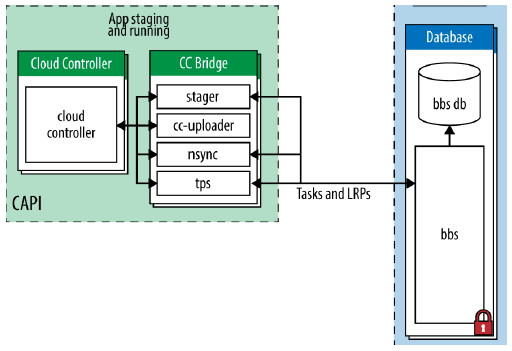
\includegraphics[width=0.75\textwidth]{fran2_1.png}
    \caption{Bulletin Boardd System en Diego subsistem}
    \label{fig:fran2_1}
\end{figure}
Se entiende por LRP los Long Range Process, procesos de larga duración, los``Desired'' son los deseados/esperados mientras que los ``Actual'' son los actuales.
Se entiende por ``Task'' las tareas.\\
El BBS (Bulletin Board System/Sistema de tablón de anuncios) es uno de los componentes de Diego. Maneja la base de datos de Diego, manteniendo una caché actualizada del estado en tiempo real del cluster de Diego, incluyendo una representación del momento de todas las Desired LRP (Los procesos de larga duración deseados), las instancias Actual LRP (Los procesos de larga duración que están actualmente en ejecución) que se están ejecutando, y las Tareas a bordo. \\
BBS está constantemente monitorizando si las LRP actuales son iguales que las LRP deseadas. Hablamos de una comparación periódica que lleva acabo BBS, y cuando las actuales son menores que las deseadas es porque existe una deficiencia y por tanto BBS se pone en funcionamiento llevando a cabo una nueva subasta de tareas y LRP’s. Cuando existe un excedente, mata instancias de tareas o LRP’s.\\
En cualquier caso, BBS tiene que llevar a cabo constantemente esta monitorización/comparación, de ahí la importancia de que estén cacheadas y mantener una caché actualizada para poder consultarlas más rápidamente y saber si hay una deficiencia o un excedente.\\
Cuando hay una deficiencia, se llama al subastador de diego el cual se encarga de asignar nuevos procesos a las máquinas virtuales y equilibrar la carga de éstas.

\subsection{Cacheo de logs y métricas en loggregator}
\begin{figure}[H]
    \centering
    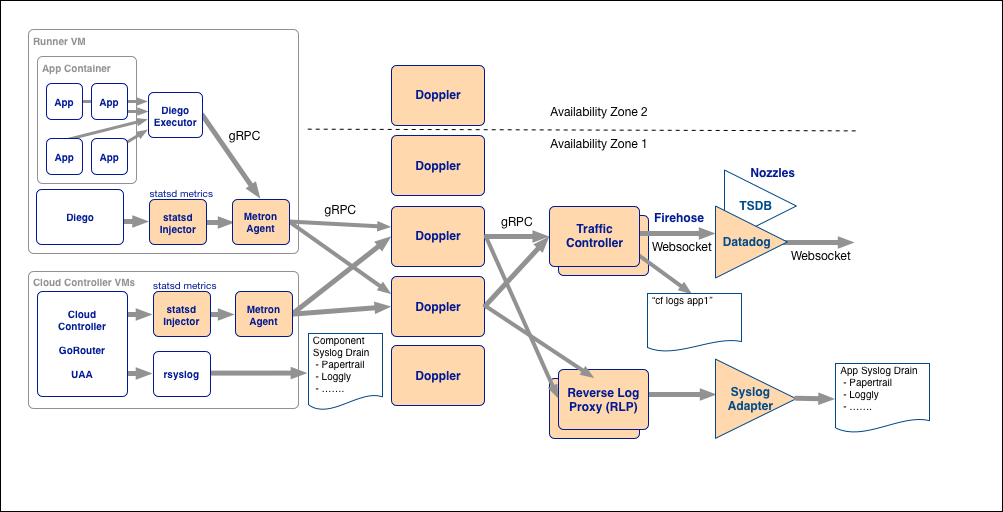
\includegraphics[width=0.75\textwidth]{fran2_2.png}
    \caption{Sistema loggregator}
    \label{fig:fran2_2}
\end{figure}
La arquitectura “Loggregator” es un subsistema de la implementación Cloud Foundry que se encarga de recopilar logs y métricas de aplicaciones de usuario que estén corriendo en una nube de Cloud Foundry. También registra logs del funcionamiento de los componentes de la implementación de Cloud Foundry.\\
Los logs y métricas son generados por los agentes Metrón (“Metron Agents”), que están colocados en las VM’s contenedoras de aplicaciones en funcionamiento.
Los logs son reportes de eventos detectados, eventos que requieren tomar alguna medida, errores que surgen y cualquier otro mensaje que el desarrollador ha querido que se generase por alguna razón intrínseca a éste.\\
Las métricas son mediciones que se hacen sobre VM’s contenedoras de aplicaciones, así como el estado de dichos contenedores.
Todos estos logs y métricas se mandan a los servidores “Dropplers” que contienen la cache, se cachean los logs y tras esto se envían al controlador de tráfico (“Traffic Controller”).
El controlador de tráfico recibe los logs de todos los servidores “Dropplers” y maneja las solicitudes de logs llevadas a cabo por el cliente interesado en dichos logs. Proporciona una API externa.\\
Luego el “Firehose” (manguera) se encarga de streamear (flujo) dichos logs y métricas provenientes del controlador de tráfico.
Los datos del flujo de la manguera no son constantes, van pasando y se van borrando, de ahí la importancia de la caché de logs ubicada en los servidores dropplers y que almacena los datos provenientes del loggregator. Dicha caché permite ver/consultar los datos desde la manguera y durante un periodo de tiempo. La cache proporciona una interfaz RESTful para recuperar los logs.
Todos estos datos pueden ser de gran utilidad, y es interesante el hecho de que puedan ser analizados por algún servicio que se encargue de ello.
La caché de registro está situada en la máquina virtual Doppler. Las dependencias de dicha caché son las siguientes:
\begin{itemize}
\item La caché de logs depende de Loggregator para ver y filtrar los logs, por lo que su fiabilidad depende del rendimiento de Loggregator. La caché de logs utiliza la memoria disponible en un dispositivo para almacenar logs y, por lo tanto, puede afectar al rendimiento del dispositivo durante períodos de alta contención de memoria.
\item La caché de logs está ubicada en las máquinas virtuales Dopplers. Acelera la recuperación de datos del sistema Loggregator, especialmente para implementaciones Cloud Foundry que cuentan con un gran número de Dopplers.
\end{itemize}

\subsection{Escalado de cache de logs}
Tal y como hemos mencionado anteriormente, se consigue una aceleración en la recuperación de logs en aquellos despliegues Cloud Foundry que cuentan con muchas VM’s Dopplers, ergo escalar la caché de logs consiste en incrementar el número de máquinas virtuales Dopplers, de esta manera aceleramos la recuperación de logs.\\
Estamos hablando de escalar la arquitectura, es decir, un componente del despliegue Cloud Foundry.

\subsection{Cacheo de microservicios con Pivotal Cloud Cache}
La proveedora de Cloud Foundry, Pivotal Software, ofrece para Pivotal Cloud Foundry una solución de caching para nuestras aplicaciones desplegadas en la nube. Esta solución está basada en el clustering. Se trata de un clúster basado en servidores ``GemFire'' para proporcionar alta disponibilidad, garantías de replicación y consistencia eventual. Cada uno de éstos   proporciona un almacén de datos consistente, de baja latencia y tolerante a fallos.

\begin{figure}[h]
    \centering
    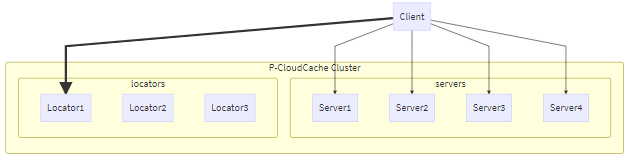
\includegraphics[width=0.75\textwidth]{fran2_3.png}
    \caption{Cluster de caches}
    \label{fig:fran2_3}
\end{figure}
Un server ``GemFire''   mantiene los datos en pares clave/valor. Cada par se llama ``entrada''. Las entradas se agrupan lógicamente en conjuntos llamados regiones. Una región es una estructura de datos de un mapa (o diccionario).
\begin{figure}[h]
    \centering
    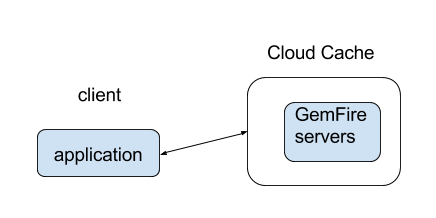
\includegraphics[width=0.75\textwidth]{fran2_4.png}
    \caption{Representación de cloud cache}
    \label{fig:fran2_4}ç
\end{figure}
El clúster de servers ``GemFire'' es escalable, aumentando así el número de servers ``GemFire'', lo que aumenta la capacidad de la memoria caché. 
\begin{figure}[h]
    \centering
    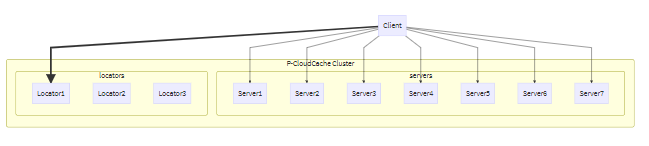
\includegraphics[width=0.75\textwidth]{fran2_5.png}
    \caption{Escalado del cache cloud cluster}
    \label{fig:fran2_5}
\end{figure}
Localizadores hay siempre tres, independientemente de que se escale o no se haga. Se llama localizador porque precisamente su función es localizar la ubicación de un server “GemFire” disponible cuando nosotros como servicio, hacemos una petición de datos a caché. Una vez que nos estemos comunicando con el server, le pedimos los datos y si éste no los tiene, le pregunta a otro server del clúster a ver si los tiene.

\begin{figure}[H]
    \centering
    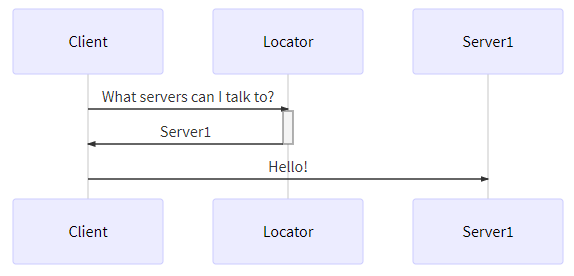
\includegraphics[width=0.75\textwidth]{fran2_6.png}
    \caption{Comunicación cliente-servidor: Localización de server GemFire}
    \label{fig:fran2_6}
\end{figure}
\begin{figure}[H]
    \centering
    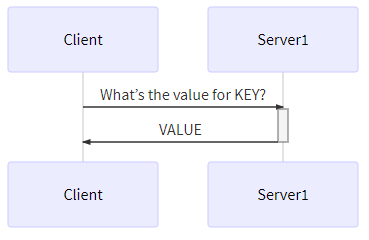
\includegraphics[width=0.75\textwidth]{fran2_7.png}
    \caption{Petición de datos a server GemFire}
    \label{fig:fran2_7}
\end{figure}
\begin{figure}[H]
    \centering
    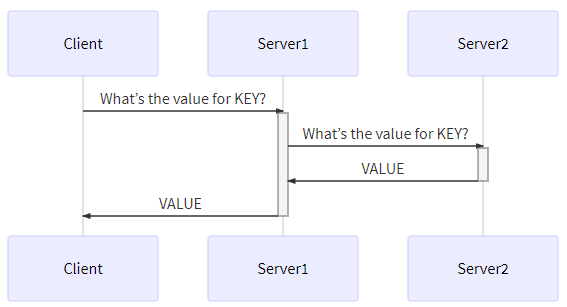
\includegraphics[width=0.75\textwidth]{fran2_8.png}
    \caption{Petición de datos de server GemFire a otro server GemFire}
    \label{fig:fran2_8}
\end{figure}

Simple pero efectivo, se trata de una arquitectura cliente-servidor

\section{Disponibilidad}%---------------Sergio

La disponibilidad es el acceso a la información y a los sistemas por personas autorizadas en el momento que así lo requieran. Los controles de seguridad utilizados para protegerlo, y los canales de comunicación protegidos que se utilizan para acceder a ella deben estar funcionando correctamente. La alta disponibilidad debe estar disponible en todo momento, evitando interrupciones del servicio debido a cortes de energía, fallos de hardware, y actualizaciones del sistema.
\subsection{Introducción a la disponibilidad en Cloud Foundry}
Cloud Foundry usado correctamente puede convertirse en la plataforma central para el desarrollo de aplicaciones así como las actividades de su implementación. Por tanto, la disponibilidad de la plataforma es fundamental para la continuidad del servicio. Los fallos se
pueden solucionar de tres formas principalmente:
\begin{itemize}
  \item Diseño para mayor resistencia y alta disponibilidad.
  \item Emplear mecanismos de respaldo y restauración.
  \item Ejecutar pruebas de verificación de la plataforma de manera constante.
\end{itemize}
\subsection{Consideraciones de alta disponibilidad}
A los usuarios finales no le importa hasta qué punto sea o no resistente su sistema, solo les preocupa que su aplicación, servicio o funcionalidad esté disponible siempre. La alta disponibilidad se mide con la percepción de los usuarios finales, que al fin y al cabo son los que experimentan percepciones negativas cuando el servicio al que intentan acceder no está disponible.\\
Tener alta disponibilidad puede ser considerado como el grado en que un componente está disponible para un usuario cuando éste lo necesite. Para conseguir una alta disponibilidad, básicamente, se necesita tener una configuración redundante de cada uno de los
componentes que haya en la infraestructura, de modo que se evite cualquier punto que provoque fallos graves, evitando así que el sistema caiga.\\
Comprender los posibles errores, como pueden ser a nivel de red, host o cluster, por ejemplo, puede ayudar a configurar y elegir una estrategia para conseguir la alta disponibilidad ya que permite evaluar cada uno de los posibles riesgos frente al coste de evitar dichos riesgos.\\
Por ejemplo, una máquina tiene una probabilidad alta de tener un fallo y por lo tanto es razonable tener una réplica; en cambio, la probabilidad de que un dentro de datos por completo quede desconectado no es tan alta y los costes asociados a la replicación, en comparación con el riesgo, son demasiado altos. Es esencial comprender qué puede fallar, el impacto de que esto ocurra así como el coste de prevenirlo antes de buscar la alta disponibilidad.\\
Una vez estudiados estos aspectos, dentro de un sistema distribuido como Cloud Foundry, se debe centrar el interés en la interconexión de los componentes para que cuando un componente individual deje de funcionar correctamente, pueda ser omitido sin perder la funcionalidad general del sistema. Cloud Foundry, junto con BOSH, promueve la capacidad de recuperación mediante la recuperación automática, que es la capacidad de superar el fallo en la aplicación, proceso o componente mediante el tratamiento y corrección de errores incorporado.\\
Cloud Foundry encara la alta disponibilidad desde arriba hacia abajo, comenzando con la disponibilidad de la aplicación y luego comprobando cada uno de los componentes del sistema que conforman la infraestructura.

\subsection{Disponibilidad del centro de datos}
Cabe destacar que antes de pensar en la alta disponibilidad de Cloud Foundry, es necesario que si centro de datos esté configurado correctamente con un nivel adecuado de alta disponibilidad.

\subsection{Ampliación de la capacidad de recuperación de Cloud Foundry}
Cloud Foundry va más allá de la simple estrategia de replicación, sino que logra la resistencia incorporada de cuatro formas clave:
\begin{itemize}
  \item Reiniciar procesos fallidos del sistemas
  \item Recrear máquinas virtuales no disponibles
  \item Implementación dinámica de nuevas instancias de aplicaciones si una aplicación deja de responder
  \item Distribución de las aplicaciones para forzar la separación de la infraestructura subyacente.
\end{itemize}
Cloud Foundry proporciona recuperación automática de aplicaciones, procesos y máquinas virtuales. Los cuatro niveles de alta disponibilidad nombrados anteriormente proporcionan resistencia dentro de los límites de una sola instalación de Cloud Foundry. Si se experimenta un fallo más amplio en el centro de datos debido a problemas en la infraestructura, una única implementación de Cloud Foundry podría quedar temporalmente inutilizable.\\
Las interrupciones del centro de datos son extremadamente raras, pero si necesita un nivel adicional de resistencia para mitigar cualquier posible fallo del centro de datos, es posible ejecutar múltiples implementaciones de Cloud Foundry en diferentes centros de datos.

\subsection{Consistencia de datos a través de servicios}
Uno de los mayores retos con la ejecución de cualquier tecnología de capa de aplicación en dos centros de datos de forma activa en ambos, es la capa de datos que sustenta la aplicación. Los servicios de respaldo de datos deben mantener la coherencia entre los dos centros de datos. Esta preocupación se explica por la teoría de que es imposible que un sistema distribuido proporcione simultáneamente garantías de consistencia, disponibilidad y tolerancia de partición. En cualquier momento, un sistema distribuido puede garantizar solo dos de los tres requisitos.\\
Mantener la consistencia de los datos en diferentes centros de datos aumenta el desafío debido a la mayor latencia cuando se intenta propagar los cambios de datos en dos ubicaciones separadas.
\begin{itemize}
  \item Si adopta un modelo de escritura simultánea en sus centros de datos, en el que devuelve una confirmación de escritura después de que se complete, la experiencia del usuario final podrá ser muy lenta. La latencia es un problema de disponibilidad y cualquier latencia de red adicional solo agravará este problema.
  \item Si adopta un modelo de escritura diferida en el que devuelve inmediatamente la confirmación de una escritura exitosa y luego intenta propagar el cambio después, corre el riesgo de que los dos almacenes de datos no queden sincronizados, dejando datos inconsistentes.
\end{itemize}
La solución aquí puede ser utilizar una capa de almacenamiento en caché local comoCassandra. El uso de una capa de datos distribuidos que garantiza la consistencia eventual en una red WAN le permite conservar los cambios localmente, permitiendo una respuesta rápida
y alta disponibilidad al usuario final. Si ocurre algún conflicto, se usan varios algoritmos de resolución de dichos conflictos para garantizar que el sistema sea finalmente coherente. Aunque ningún sistema consistente es infalible al cien por cien, se proporciona una solución sólida al problema de la consistencia planteado.

\subsection{Copias de seguridad}
Hay veces que es posible que necesite restaurar completamente su entorno. Esto podría deberse a cualquiera de estas situaciones:
\begin{itemize}
  \item Creación de una copia de una implementación existente para crear un entorno completamente nuevo.
  \item Motivos de mantenimiento, como cambiar o actualizar su red, servidor o capa de almacenamiento.
  \item Recuperación de un ataque malicioso en todo el centro de datos que provoca un fallo catastrófico.
\end{itemize}
Hay varios proyectos que existen para respaldar y restaurar Cloud Foundry, como por ejemplo:
\begin{itemize}
  \item cf-converger de Engineer Better
  \item cfops de Pivotal Services
\end{itemize}
Para restaurar su entorno, primero debe crear una copia de seguridad de la capa de datos. Al pensar en Cloud Foundry desde una perspectiva de recuperación ante desastres, debe pensar en el sistema distribuido como un conjunto de discos persistentes que contienen lo siguiente:
\begin{itemize}
  \item El CCDB.
  \item La base de datos de la UAA.
  \item El BBS.
  \item El DB BOSH.
  \item El blobstore o servidor NFS.
  \item Configuración.
  \item Cualquier otra capa de persistencia centrada en la aplicación.
\end{itemize}
La capa de persistencia es Cloud Foundry desde una perspectiva de recuperación de desastres; Todo lo demás, todos los procesos en ejecución, pueden volver a conectarse fácilmente.

\subsection{Disponibilidad de Cloud Foundry}
La copia de seguridad de Cloud Foundry suspenderá las escrituras mientras dure la copia de seguridad. Esto es importante porque no puede escribir simultáneamente en una base de datos y mantener la integridad de la copia de seguridad de la base de datos. La suspensión de las escrituras hará que su base de datos se convierta en de solo lectura durante la copia de seguridad. Las aplicaciones no funcionarán durante este tiempo.\\
Recuperar BOSH es el primer paso para recuperar cualquier entorno de Cloud Foundry que se encuentre offline. Por lo tanto, es vital que tome instantáneas regulares de la base de datos BOSH. Es mejor usar una base de datos externa como MySQL en clúster o AWS-RDS y un
blobstore externo como Amazon S3. Sin embargo, si utiliza la base de datos interna de BOSH,hay algunos pasos adicionales necesarios para realizar una copia de seguridad y restaurar la base de datos interna y el blobstore de BOSH.\\
Puede usar los siguientes pasos para hacer una copia de seguridad de la base de datos interna y el blobstore de BOSH:

\begin{enumerate}
  \item Usando SSH, conéctese a BOSH: \$ ssh -i key vcap@boship
  \item Conviértete en root: \$ su -(usa tus credenciales de VM)
  \item Ejecutar \$ monit summary para ver todos los procesos BOSH
  \item Ejecutar \$ monit stop all para detener limpiamente todos los procesos BOSH
  \item Tome una instantánea del volumen de disco persistente BOSH
\end{enumerate}

Estos son los pasos para restaurar la base de datos interna y el blobstore de BOSH:
\begin{enumerate}
  \item Usando su manifiesto bosh.yml original , reconstruya BOSH. Esto crea un nuevo disco persistente vacío.
  \item Repita los pasos 1 a 4 del procedimiento de copia de seguridad. Deberá detener todos los procesos antes de desconectar el disco persistente.
  \item Desacoplar el disco persistente (eliminándolo).
  \item Cree un nuevo volumen a partir de su instantánea de volumen de disco y luego adjunte manualmente el nuevo volumen a la máquina virtual BOSH.
  \item Iniciar todos los procesos de nuevo. BOSH ahora tendrá el mismo UOS BOSH (porque está almacenado en la base de datos).
\end{enumerate}
Una vez que haya restaurado con éxito BOSH, BOSH debería restaurar con éxito la implementación de Cloud Foundry, asumiendo que ha utilizado una base de datos externa y accesible y blobstore para los otros componentes.





%---------------------------------------------------------------------------------------
\section{Mantenimiento}
\subsection{Mantenimiento general}
\subsubsection{Mantenimiento del datacenter}
Respecto al mantenimiento del datacenter en el que se encuentra nuestra instancia de Cloud Foundry nos encontramos con un mantenimiento general tal y como hemos visto en la asignatura.\\
Deberemos de tener en cuenta los sitemas de alimentación eléctrica, extinción de incendios, climatización asi como el equipamiento de comunicaciones y televigilancia. Debido a que todos estos temas se alejan del objetivo de este trabajo de investigación se recomienda la lectura de la bibliografia para adquirir mas conocimiento al respecto \cite{cpdbib}.

\subsubsection{Mantenimiento del hardware y software}
En cuanto al mantenimiento del hardware nos encontramos también con un mantenimiento general que garantize el correcto funcionamiento de los equipos.\\
Respecto al software, el mantenimientos será, una vez más, general. Ya que CF se monta sobre una estructura Linux se entiende que los administradores de los sistemas tendrán que mantener estos sistemas funcionando asi como realizar actualizaciones de paquetes, de kernels, escrutinio de logs, etc.\\
Una vez mas, como este tema se aleja del objetivo de este trabajo se recomienda la lectura de la bibliografia \cite{redhatSysadminguide}.

\subsection{Mantenimiento específico de Cloud Foundry}
\subsubsection{Testing con Inigo y CATs}
Inigo es una suite de test que se le pueden pasar a todos los componentes Diego para de esta forma asegurarnos de que todo se ejecuta correctamente.\\
CATs, sigla de CF Acceptance Test es, al igual que Inigo, otra suite de tests que se ejecutan con cfdot CLI y mediante peticiones curl.
\subsubsection{cfdot CLI}
cfdot, cuyo nombre completo es CF Diego Operator Toolkit es una CLI que nos permite interactuar con un despliegue de Diego. Mediante esta herramienta podremos lanzar comados que cambien en comportamiento de los llamados LRP (Long-Running Process).\\
Un ejemplo de lo que podemos realizar sería crear y retirar distintos LRP mediante indice o uid asi como listar y modificar distintas tareas a realizar por los componente Diego.

\subsection{Opciones en desarrollo}
\subsubsection{admin-ui}
Existen además varias opciones que se encuentran en desarrollo, una de las mas interesantes es Admin-UI, que pretende crear una interfaz gráfica que pueda controlar aspectos importantes de un despliegue de CF. En la figura \ref{fig:admin-ui} podemos ver la interfaz gráfica de esta herramienta.

\begin{figure}[h]
    \centering
    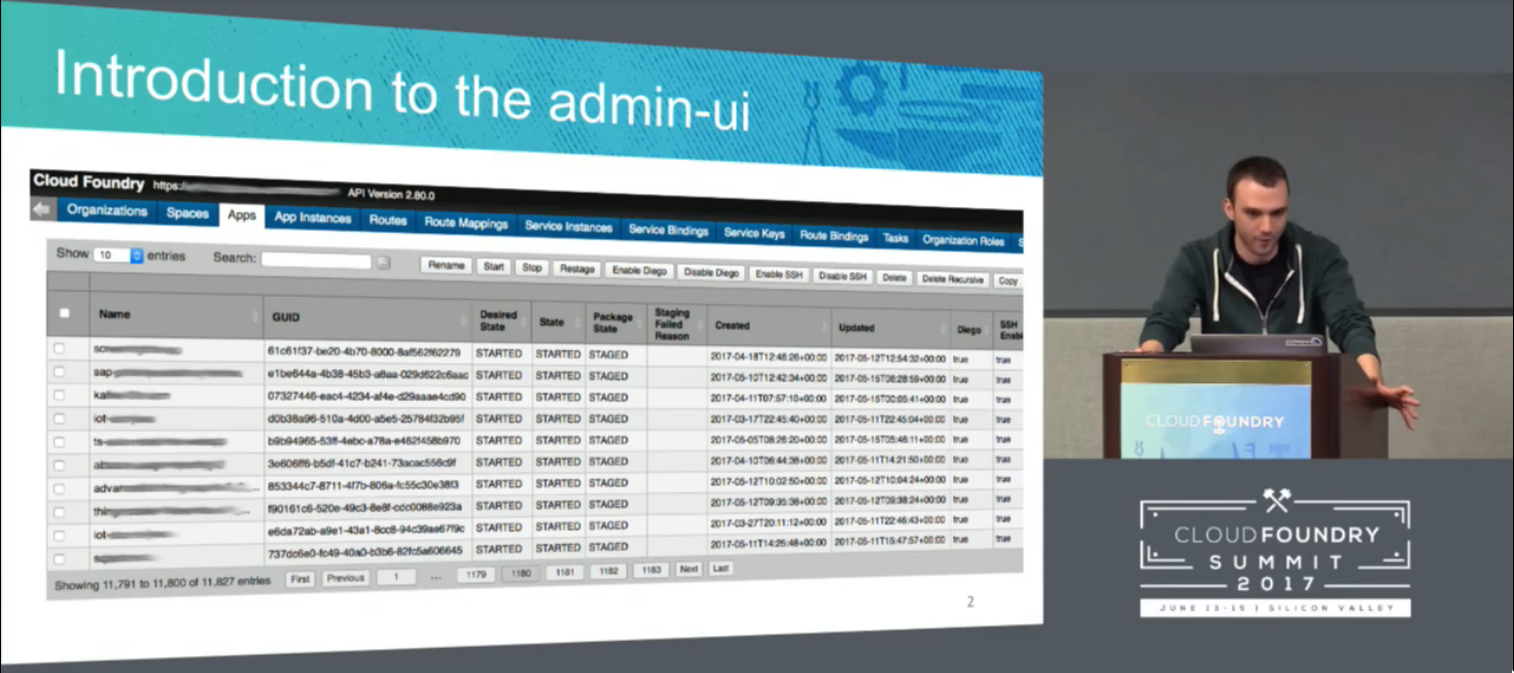
\includegraphics[width=0.9\textwidth]{fotogramaCharlaUI.png}
    \caption{Fotograma extraido de la charla `Deploy the admin-ui as a CloudFoundry application' en el que se muestra la interfaz gráfica de admin-ui}
    \label{fig:admin-ui}
\end{figure}
%---------------------------------------------------------------------------------------


\section{Uso en el mundo real}

Los usos en el mundo real hacen referencia a quien, donde y como se hace uso de la plataforma Cloud Foundry en el ambitó práctico en base a lo que esta plataforma ofrece y a sus posibles aplicaciones en el ambito laboral y personal.

El uso de Cloud Foundry  en el mundo real es el de servir como plataforma de desarrollo de aplicaciones a emprendedores que necesitan un lugar donde poder implementar y probar sus aplicaciones, lo cual pueden hacer tanto en la nube con Cloud Foundry.com, como en local con Micro Cloud Foundry dando la seguridad de que si funciona en uno funcionará en el otro y además desean centrarse solo en ese aspecto y no tener que ocuparse por la infraestructura de las capas inferiores ya que Cloud Foundry esta diseñado para ofrecer apoyo y un gran nivel de abstracción sobre la infraestructura.

Además de que al ser una plataforma de codigo abierto, es gratuita lo cual es una ventaja para los desarrolladores jovenes que no tienen grandes ingresos. También Cloud Foundry gestiona el espacio en el que trabajan los desarrolladores lo cual es una ventaja para estos ya que al estar separados, no hay riesgo de que se junte con los proyectos de otros desarrolladores, ni de que nadie lo vea hasta que sea publicado.

Y también es posible su uso para empresas más grandes gracias a Pivotal Cloud Foundry que es una variante de Cloud Foundry diseñada especialmente para las empresas ofreciendo una plataforma agil, flexible y eficiente gracias al uso de contenedores que mejoran el depliege, ejecución y gestion de aplicaciones.

%---------------------------------------------------------------------------------------
\section{Conclusiones}
En resumen Cloud Foundry es una plataforma gratuita, de código libre, creada para que los desarrolladores puedan centrarse en la creación e implementación de aplicaciones sin tener que preocuparse por la infraestructura inferior, que además posee una alta disponibilidad a través de la interconexión de sus componentes, se basa en un sistema distribuido con contenedores, tiene replicaciones con centros de datos múltiples y un sistema de cache para reducir el tiempo de ejecución.\\

Por lo que en conclusión Cloud Foundry es una plataforma para desarrollo de aplicaciones con un buen diseño tanto en cuanto a su estructura física como en su estructura de software, una buena administración de recursos y en general una aplicación funcional y operativa para cualquiera que desee usarla.

\begin{thebibliography}{99}

\bibitem{cf_architecture}
Cloud Foundry Foundation 2018,
\textit{Cloud Foundry Components}
\href{https://docs.cloudfoundry.org/concepts/architecture/index.html}{Documentación web de Cloud Foundry}

\bibitem{cf_book_1}
Winn, D. (2016). \textit{Cloud foundry: the cloud-native platform.}
(First edition.). Beijing, China: O’Reilly.

\bibitem{cf_book_2}
Winn, D. (2017). \textit{Cloud Foundry: the definitive guide: develop, deploy, and scale.} First Edition. Beijing, China: O’Reilly.

\bibitem{cf_book_3}
Farmer, R., Jain, R., y Wu, D. (2017). \textit{Cloud Foundry for developers: deploy, manage, and orchestrate cloud-native applications with ease.} Birmingham, England: Packt.s.

\bibitem{CharlaUI}
Michael Grifalconi. \textit{Deploy the admin-ui as a CloudFoundry applications.}
\href{https://www.youtube.com/watch?v=9Np7swZN-4g}{Cloud Foundry Youtube channel.}

\bibitem{runningCF}
Cloud Foundry Foundation 2018.
\textit{Running Cloud Foundry}
\href{ https://docs.cloudfoundry.org/running/index.htm}{Documentación web de Cloud Foundry}

\bibitem{adminguideCF}
Cloud Foundry Foundation 2018.
\textit{Administering and Operating Cloud Foundry }
\href{https://docs.cloudfoundry.org/adminguide/}{Documentación web de Cloud Foundry}

\bibitem{tema4CIMSI}
F. Gómez, A. Crespo, Daniel Cascado Caballero, Rosa Yánez Gómez, Mª José Morón Fernández.
\textit{TEMA 4: Mantenimiento en TI}
.Temario de la asignatura CIMSI.

\bibitem{redhatSysadminguide}
Marie Doleželová, Marc Muehlfeld, Stephen Wadeley, Tomáš Čapek, Jaromír Hradílek, Douglas Silas, Jana Heves, Petr Kovář, Peter Ondrejka, Petr Bokoč, Martin Prpič, Adam Kvítek, Eliška Slobodová, Eva Kopalová, Miroslav Svoboda, David O'Brien, Michael Hideo, Don Domingo, John Ha.
\textit{System Administrator's Guide} \href{https://access.redhat.com/documentation/en-US/Red_Hat_Enterprise_Linux/7/html-single/System_Administrators_Guide/}{Documentación web de RedHat}

\bibitem{cpdbib}
Juan F. Gómez Fernández, Adolfo Crespo Márquez. \textit{Maintenance Management in Network Utilities, Framework and Practical Implementation}. 2012 Springer Verlag UK. London.

\end{thebibliography}
\end{document}
